\section{Extensions}

We will now explore the potential application of the one-step ahead predictor formula with the Kalman Filter in various contexts beyond its original domain.

\subsection{Multi-step prediction}
Assuming that $\hat{\mathbf{x}}(t+1\mid t)$ is known, the $k$-step ahead prediction can be straightforwardly computed. 
Given $\hat{\mathbf{x}}(t+1\mid t)$, we can derive:
\[\begin{cases}
    \hat{\mathbf{x}}(t+k\mid t)=\mathbf{F}^{k-1} \hat{\mathbf{x}}(t+1\mid t) \\
    \hat{\mathbf{y}}(t+k\mid t)=\mathbf{H} \hat{\mathbf{x}}(t+k\mid t)
\end{cases}\]

\subsection{Filtering}
The filtering process, denoted as $\hat{\mathbf{x}}(t\mid t)$, aims to estimate the current state of the system given available measurements up to time $t$. 
Assuming that $\hat{\mathbf{x}}(t+1\mid t)$ is known, we can compute $\hat{\mathbf{x}}(t\mid t)$ using different formulations based on the properties of the system matrix.

\paragraph*{Straightforward solution}
If the matrix $\mathbf{F}$ is invertible, we have a straightforward solution:
\[\hat{\mathbf{x}}(t\mid t)=\mathbf{F}^{-1} \hat{\mathbf{x}}(t+1\mid t)\]

\paragraph*{Filter formulation}
In special cases where $\mathbf{F}$ is not invertible, we use the filter formulation of the Kalman Filter:
\[\begin{cases}
    \hat{\mathbf{x}}(t\mid t)=\mathbf{F}\hat{\mathbf{x}}(t-1\mid t-1)+\mathbf{K}_0(t)\mathbf{e}(t) \\
    \hat{\mathbf{y}}(t\mid t-1)=\mathbf{H}\hat{\mathbf{x}}(t\mid t-1) \\
    \mathbf{e}(t)=\mathbf{y}(t)-\hat{\mathbf{y}}(t\mid t-1) \\
    \mathbf{K}_0(t)=\left(\mathbf{P}(t)\mathbf{H}^T\right)\left(\mathbf{HP}(t)\mathbf{H}^T+V_2\right)^{-1} \\
    \mathbf{P}(t+1)=\left(\mathbf{FP}(t)\mathbf{F}^T+V_1\right)-\left(\mathbf{FP}(t)\mathbf{H}^T+V_{12}\right)\left(\mathbf{HP}(t)\mathbf{H}^T+V_{2}\right)^{-1}\left(\mathbf{FP}(t)\mathbf{H}^T+V_{12}\right)^T
\end{cases}\]
The initial condition for the filter is $\hat{\mathbf{x}}(1\mid 1)=\mathbf{x}_0$. 
The equation for $\mathbf{K}_0(t)$ is referred to as the filter gain.
This formula is valid only when $V_{12}=0$, which is typically true in practice.

\paragraph*{Gains}
There's a distinction between two gains when $V_{12}=0$: 
\begin{itemize}
    \item Prediction gain: $\mathbf{K}(t)=\left(\mathbf{FP}(t)\mathbf{H}^T+V_{12}\right)\left(\mathbf{FP}(t)\mathbf{H}^T+V_2\right)^{-1}$.
    \item Filter gain: $\mathbf{K}_0(t)=\left(\mathbf{P}(t)\mathbf{H}^T\right)\left(\mathbf{HP}(t)\mathbf{H}^T+V_2\right)^{-1}$.
\end{itemize}
The primary difference lies in the initial $\mathbf{F}$, which is absent in the filter gain equation.

\subsection{Exogenous input}
Graphically, the Kalman Filtering process with an eXogenous input $\mathbf{Gu}(t)$ is illustrated as follows:
\begin{figure}[H]
    \centering
    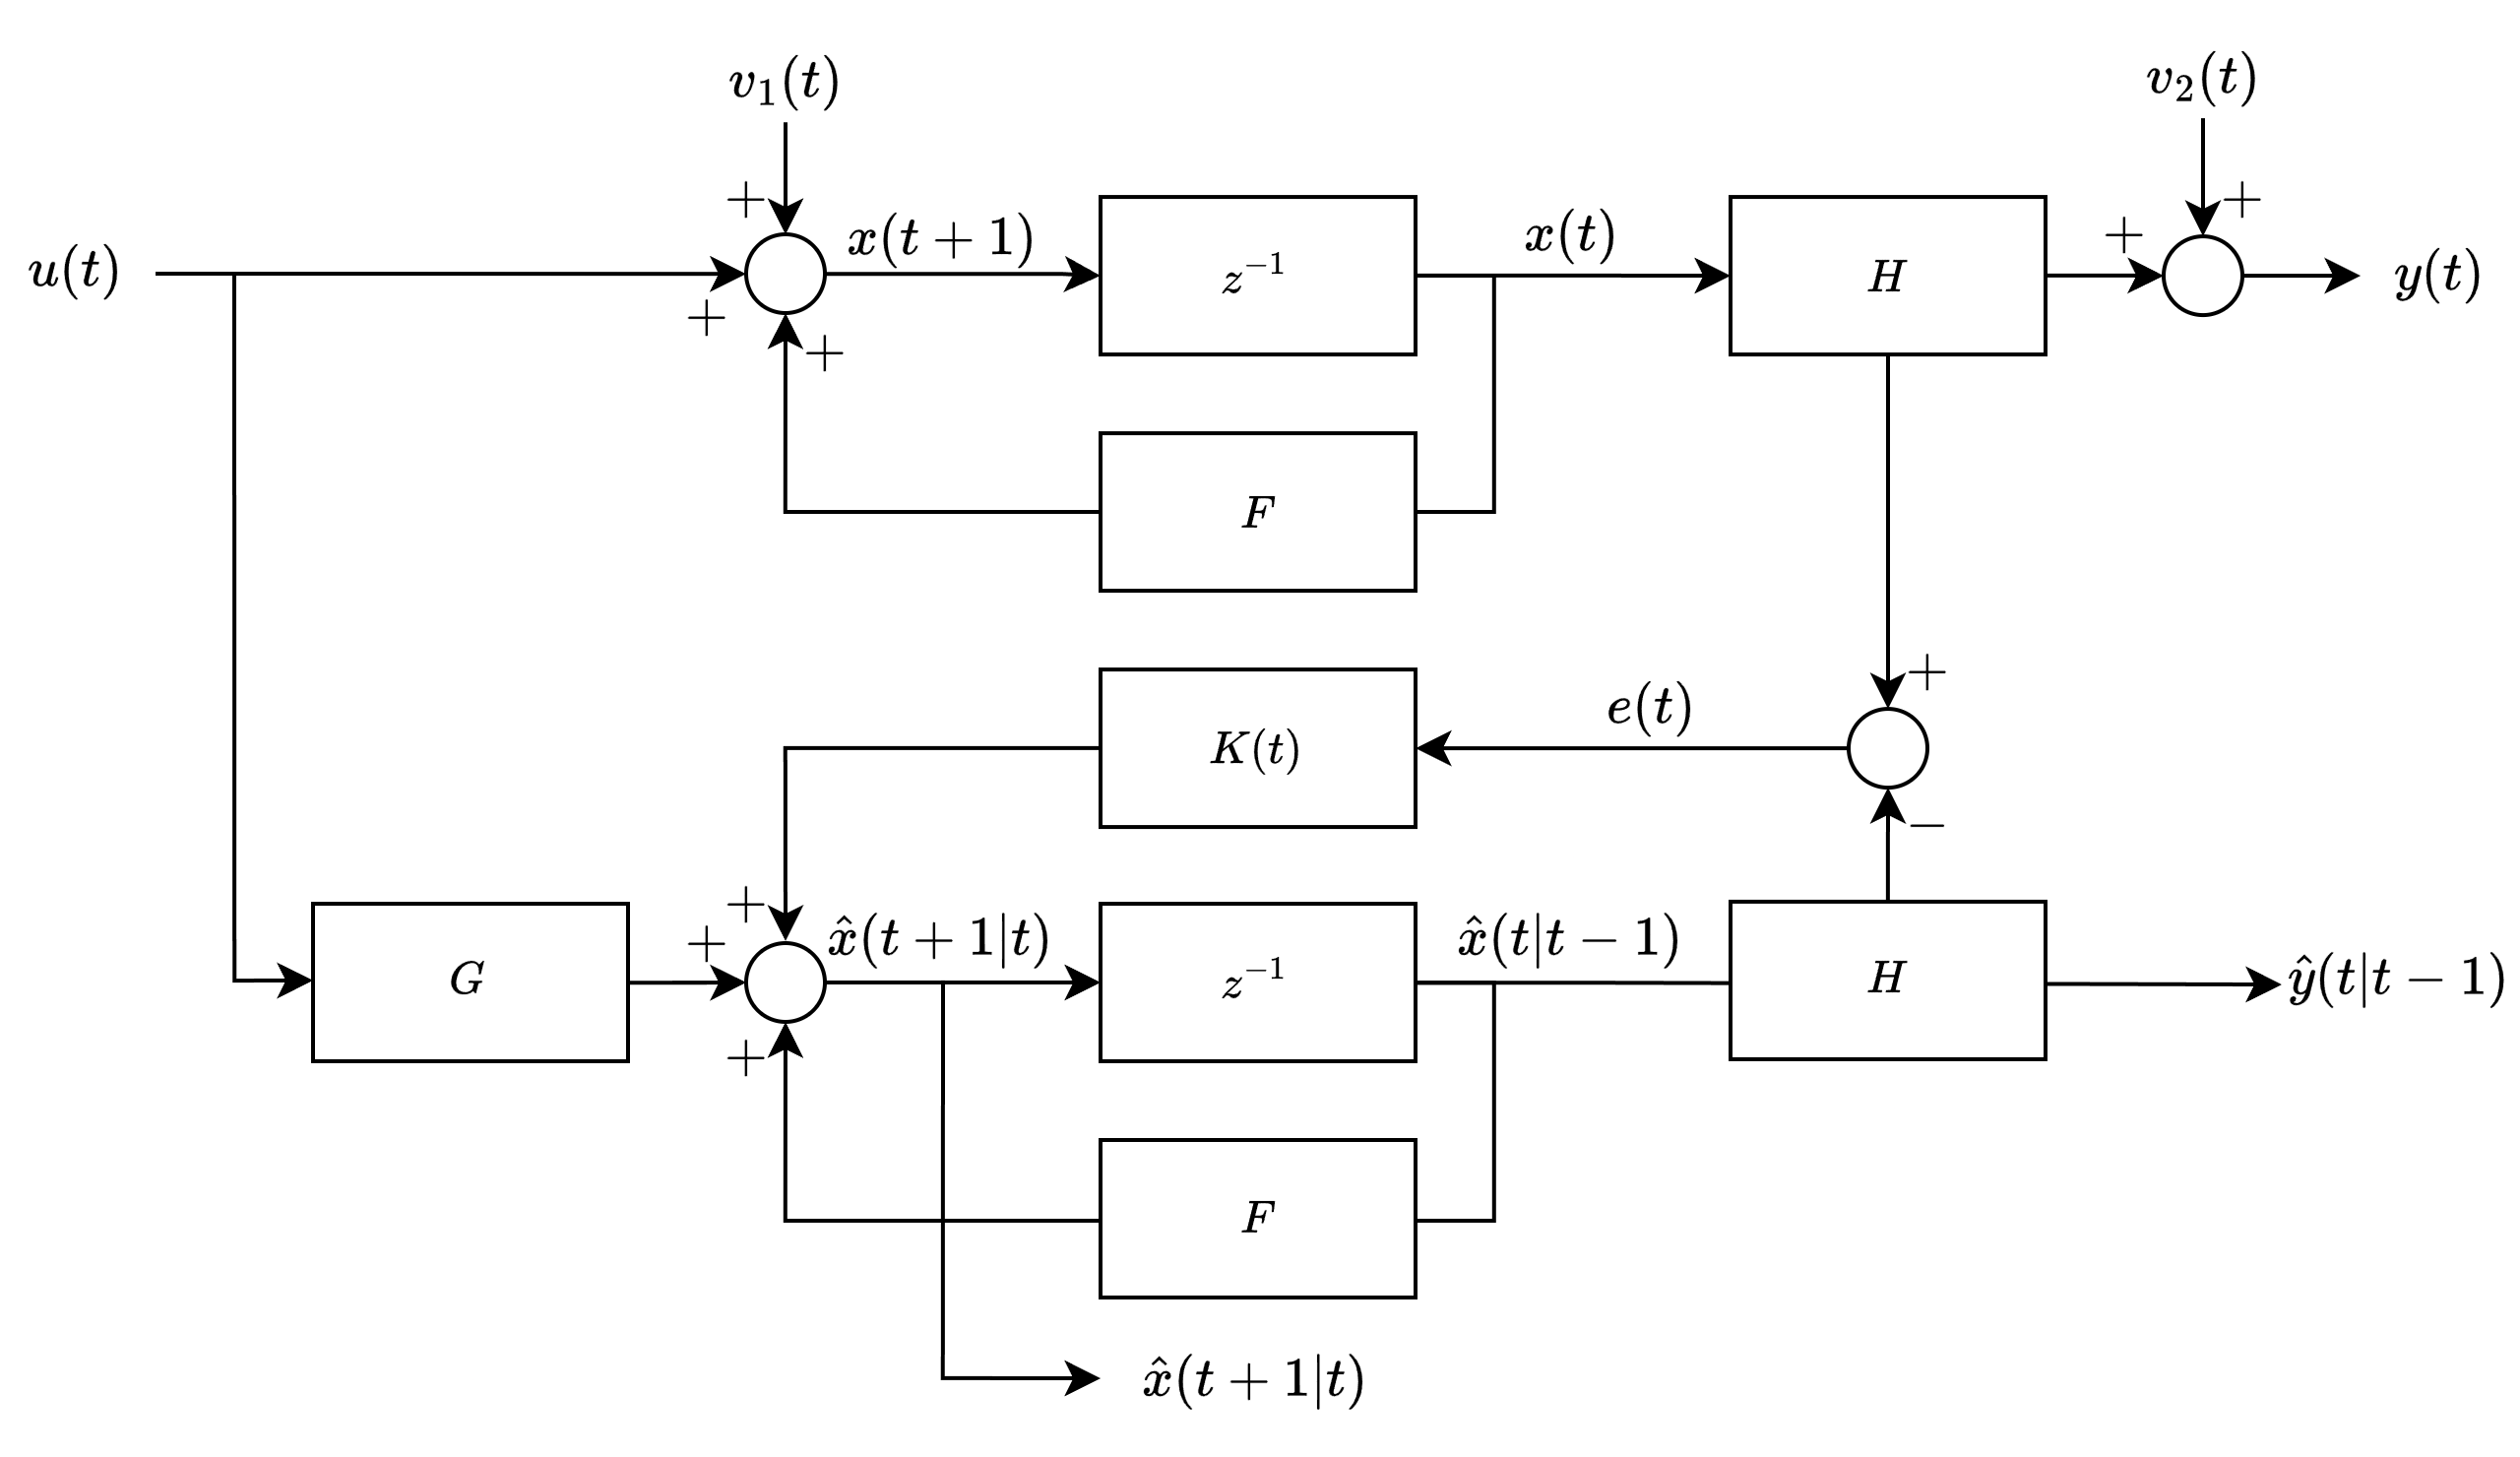
\includegraphics[width=0.75\linewidth]{images/ke.png}
    \caption{Kalman Filtering with eXogenous input}
\end{figure}
Notably, the $\mathbf{K}(t)$ and $\mathbf{P}(t)$ terms remain unchanged from the formulas without $\mathbf{Gu}(t)$. 
This intuitively makes sense because $\mathbf{Gu}(t)$ does not introduce additional uncertainty into the system; rather, it represents a deterministic component added to the system. 
Consequently, the state prediction error $\mathbf{P}(t)$ remains unaffected.

\subsection{Time-variant systems}
Consider a system represented by the following equations, where all matrices are time dependent:
\[\begin{cases}
    \mathbf{x}(t+1)=\mathbf{F}(t)\mathbf{x}(t)+\mathbf{G}(t)\mathbf{u}(t)+\mathbf{v}_1(t) \\
    \mathbf{y}(t)=\mathbf{H}(t)\mathbf{x}(t)+\mathbf{v}_2(t)
\end{cases}\]
In this scenario, even with time-variance in the system matrices, the Kalman Filter equations remain identical to those of time-invariant systems.